\section{Scaling \ourapproach to a Real-World Automated Valuation Model}\label{sec:avm}

 This appendix details the deployed-AVM study summarised in \cref{sec:evaluation}.

The synthetic archetypes of \cref{sub:synthetic}, the AC benchmark of
\cref{sec:ac_benchmark}, and the SIR benchmark of \cref{sec:sir_benchmark} all
controlled the model and the ground truth, so that \ourapproach could be judged
against an analytic verdict or a competing AC enumeration. Here we drop both,
applying \ourapproach to a deployed valuation model for residential housing on
which neither ground truth nor exact AC enumeration is available. Disclosure
constraints on the trained model and its training data prevent a quantitative
accuracy comparison on this system, so the quantitative validation of
\ourapproach{} lives entirely in the controlled synthetic benchmark of
\cref{sub:synthetic}. The role of this appendix is correspondingly narrow: to
report (i) that \ourapproach{} is computationally feasible at production scale on a
model with millions of training points, and (ii) that the qualitative SHAP-vs-PCI
divergence observed in \cref{sec:shap_examples} persists when the model is a real
trained one: the shape of the two attribution distributions and where
attribution mass lands, not the substantive content of the features they assign to.

\paragraph{Setting.}
The unit of analysis is a residential property transaction. \ourapproach is run
against the full country-level production AVM; what we show here is an
illustrative prototype based on the state of New York rather than
the full national model structure, which we cannot disclose in detail. The NY
prototype shares the architecture and the causal-kernel construction described
below with the full system but is smaller in scope and DAG complexity. The
computational-feasibility claim refers to the full national system; the
qualitative SHAP-vs-PCI behaviour we illustrate is a property of the shared
architecture and carries over from the prototype. The
outcome variable $y$ is the (log-epsilon-standardized) sale price. Transactions are
described by a set of categorical variables $x_{cat} = x_{1}, \dots, x_k$ and continuous
(transformed) variables\footnote{Usually log-epsilon-standardized,
standardized-truncated, or standardized.} $x_{con} = x_{k+1}, \dots, x_n$.

\paragraph{Causal model.}
A causal DAG $\mathcal{G}$ expresses our causal assumptions about the relationships between
variables. We wrote it manually in collaboration with domain experts, then refined it by
adding edges to break implied conditional independencies not upheld by the
data. The simplified NY-prototype DAG has 25 nodes and 99 edges; topology with anonymised node
labels is shown in Figure~\ref{fig:avm_dag}; the full national DAG is larger and is
not shown. As demonstrated in \cref{sec:ac_benchmark}, even the prototype is
already large enough that exact actual-causality enumeration is computationally
infeasible, and the same conclusion applies a fortiori to the national system.

Variables $x_i$ are drawn from distributions $\mathrm{Dist}_i$ parameterized by functions
$f_i(\mathrm{pa}_i, \varphi_i)$ of the parent variables
$\mathrm{pa}_i$\footnote{For root nodes, $\mathrm{pa}_i$ is empty.}:
$x_i \sim \mathrm{Dist}_i(f_i(\mathrm{pa}_i, \varphi_i))$. We call these distributions
\emph{causal kernels}. The distributions are either (truncated) normal or categorical; we choose the
family based on the domain of the variable it models. The functions $f_i$ are deep
neural networks with parameters $\varphi_i$, which we optimize using cross-entropy
loss for categorical distributions and average negative log likelihood for
continuous distributions. The outcome is modeled by a sparse variational
Gaussian Process (SVGP; \citealp{titsias2009variational,hensman2013gaussian}),
$x_{gp} = (x_{con}, \eta(x_{cat}, \varphi_{cat}))$,
$y \sim \mathcal{SVGP}\!\left(\mu(x_{gp}, \varphi_\mu), \kappa(x_{gp}, \varphi_\kappa)\right)$,
where $\eta$ is a linear embedding of the categorical variables into the continuous
space, jointly optimized with the GP.

\begin{figure}[htbp]
\centering
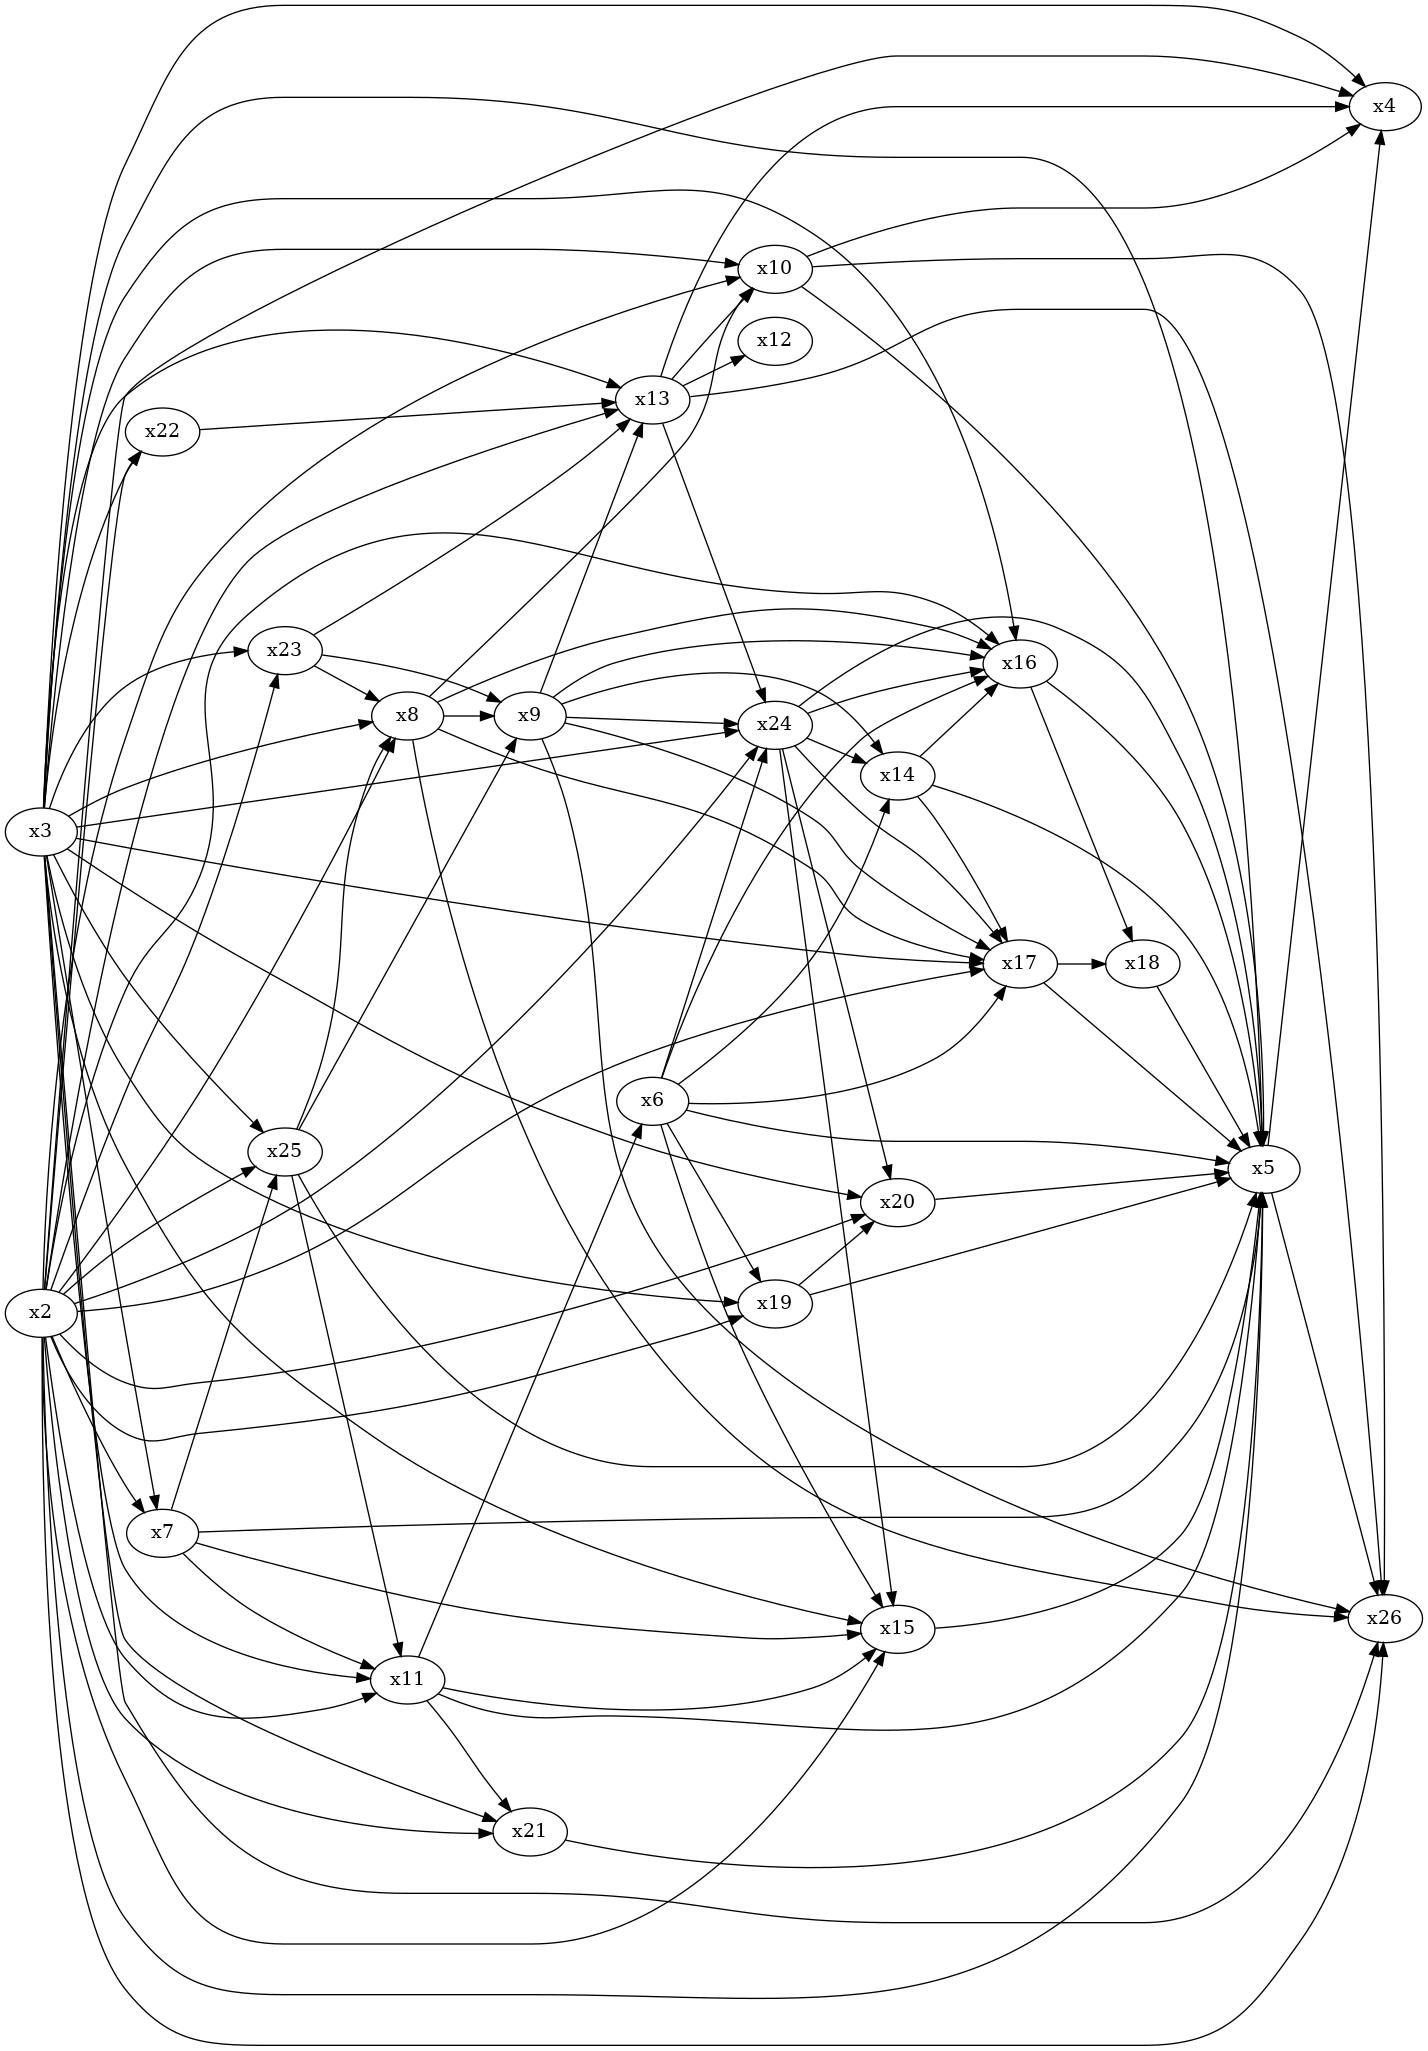
\includegraphics[width=0.85\linewidth]{figures/anonymized_upstream_structure.png}
\caption{Topology of the AVM causal DAG (NY-prototype version), with node labels
anonymised. The graph has 25 nodes and 99 edges; the full national DAG is larger
and is not shown. Several variables sit deep in the DAG with high in-degree; these
are the nodes towards which SHAP allocates disproportionate attribution mass (see
Figure~\ref{fig:eval_avm}).}
\label{fig:avm_dag}
\end{figure}

\paragraph{Feasibility at production scale.}
To apply \ourapproach we transform the model as described in
Section~\ref{sec:causal_impact} and evaluate the impact of features from a list of
potential causal suspects, using the absolute difference impact score of
Example~\ref{ex:absolute_score}. We draw Monte Carlo samples from the expanded model.
Conditioning on a given suspect $X_i$ being active gives us a sample of the scores
corresponding to that feature, which we use to estimate the expected value thereof. The
estimation converges at around \num{25000} samples; for a batch of 50 data points this
takes around 60 minutes on commodity hardware. We need to sample only once; we can then reuse the samples to compute the
attribution score of any suspect. This
establishes that the method is computationally tractable at production scale, not a
foregone conclusion, since the expanded-model construction in
Section~\ref{sec:causal_impact} introduces additional latent dimensions per suspect and
per witness.

\paragraph{Qualitative comparison to SHAP.}
We compare \ourapproach attributions to SHAP scores \citep{lundberg2017unified} on the
same trained model. SHAP heavily weights variables that are downstream of many other
variables in the causal graph, effectively assigning attribution to what amount to
summary statistics of the outcome. \ourapproach distributes attribution more evenly
across the upstream causal structure. The pattern is consistent with what
Section~\ref{sec:shap_examples} establishes on controlled examples: SHAP's observational
marginalisation allocates weight differently from intervention-and-witness-based PCI
scores, and on a deep DAG this difference manifests as concentration on
summary-statistic-like nodes. Figure~\ref{fig:eval_avm} shows the two attribution
distributions with anonymised feature labels; here we can report the shape of
the two distributions, not which features they assign to.


